\documentclass[conference]{IEEEtran}

\usepackage{graphicx}
\usepackage{hyperref}
\usepackage{xspace}
\usepackage{listings}
\usepackage[usenames, dvipsnames]{color}
         

\graphicspath{{./img/}}

\hyphenation{op-tical net-works semi-conduc-tor}


\lstset{language=Python}

\definecolor{LightGray}{RGB}{250,250,250}

\lstdefinestyle{custompython}{
	captionpos=b,                    % sets the caption-position to bottom
	% frame=tb,
	xleftmargin=\parindent,
	language=Python,
	basicstyle=\footnotesize\ttfamily,
	keywordstyle=\bfseries\color{MidnightBlue},
	stringstyle=\color{PineGreen},
  	commentstyle=\color{Magenta},
  	backgroundcolor=\color{LightGray}
}


\newcommand{\tool}{Flask Dashboard\xspace}
\newcommand{\zee}{Zeeguu\xspace}
\newcommand{\git}{\texttt{git}\xspace}
\newcommand{\install}{{\small \texttt{pip install flask\_dashboard}}\xspace}
\newcommand{\activeUserCount}{two hundred\xspace}
\newcommand{\code}[1]{\texttt{#1}\xspace}
\newcommand{\perspective}[1]{{\small {\texttt{#1}}\xspace}}

\usepackage{fourier-orns}

\definecolor{myred}{RGB}{230, 20, 70}
\definecolor{mygreen}{RGB}{60, 180, 75}


\newcommand{\niceseparator}
	{
		\begin{center}
  		% $\ast$~$\ast$~$\ast$
  		% $\clubsuit$~$\clubsuit$~$\clubsuit$
  		\leafleft
		\end{center}
	}

% Endpoint Names 
%\newcommand{\epDecoration}[1]{{\small {\bf #1}}\xspace}
\newcommand{\epDecoration}[1]{\code{#1}}

\newcommand{\epTranslations}{{\color{myred} \epDecoration{api.get\_possible\_translations}}\xspace}
\newcommand{\epOutcome}{\epDecoration{api.report\_exercise\_outcome}}
\newcommand{\epFeedItems}{\epDecoration{api.get\_article\_difficulties}}



% Author Comments / Discussion

\definecolor{mlcolor}{RGB}{140, 140, 205}
\definecolor{vacolor}{RGB}{255, 0, 255}

\newcommand{\ml}[1]{ 
	{\footnotesize \color{mlcolor}ML: #1}
	}

\newcommand{\va}[1]{ 
	{\footnotesize \color{vacolor}VA: #1}
}


\newcommand{\mltp}[1]{\ml{Thijs, Patrick: #1}}
\newcommand{\mlv}[1]{\ml{Vasilios: #1}}

\definecolor{todocolor}{RGB}{200, 140, 160}

\newcommand{\todo}[1]{ 
	{\footnotesize \color{todocolor}Todo: #1}
	}

\newcommand{\Fref}[1]{Fig.~\ref{#1}}
\newcommand{\Sref}[1]{Sec.~\ref{#1}}




\begin{document}
%
\title{A Low-Effort Analytics Platform for Visualizing Evolving Flask-Based Python Web Services}
% Alternative Titles: The Importance of Visualization in the Performance Monitoring of Python Web Services


% author names and affiliations
% use a multiple column layout for up to three different
% affiliations
%\author{\IEEEauthorblockN{Michael Shell}
%\IEEEauthorblockA{School of Electrical and\\Computer Engineering\\
%Georgia Institute of Technology\\
%Atlanta, Georgia 30332--0250\\
%Email: http://www.michaelshell.org/contact.html}
%\and
%\IEEEauthorblockN{Homer Simpson}
%\IEEEauthorblockA{Twentieth Century Fox\\
%Springfield, USA\\
%Email: homer@thesimpsons.com}
%\and
%\IEEEauthorblockN{James Kirk\\ and Montgomery Scott}
%\IEEEauthorblockA{Starfleet Academy\\
%San Francisco, California 96678--2391\\
%Telephone: (800) 555--1212\\
%Fax: (888) 555--1212}}

\author{
\IEEEauthorblockN{Patrick Vogel, Thijs Klooster, Vasilios Andrikopoulos, Mircea Lungu}\\
Johann Bernoulli Institute for Mathematics and Computer Science\\
University of Groningen, Netherland\\
Email: \{t.klooster.1,p.p.vogel\}@student.rug.nl, \{v.andrikopoulos,m.f.lungu\}@rug.nl 
}

% make the title area
\maketitle

\begin{abstract}

  Tens of thousands of web applications are written in Flask, a Python-based web framework. Despite a rich ecosystem of extensions, there is none that supports the developer in gaining insight into the evolving performance of their service. In this paper, we introduce \tool, a library that addresses this problem. We present the ease with which the library can be integrated in an already existing web application, discuss some of the visualization perspectives that the library provides and point to some future challenges for similar libraries.

\end{abstract}

% no keywords

\IEEEpeerreviewmaketitle



\section{Introduction}

%Every system is a distributed system nowadays \cite{cavage2013there}. Indeed a very large number of applications and web applications are nowadays implemented as two-tier architectures with a front-end implemented with web technologies and a service back-end.
%\ml{I'm not completely happy with this paragraph}
{\em There is no getting around it: you are building a distributed system} argues a paper from almost half a decade ago \cite{cavage2013there}. Indeed, since then, even the simplest second-year student project is a web application implemented as two-tier architectures with a front-end implemented in Javascript and HTML 5 and a service backend, usually a REST API.

% \hfill mds
Many contemporary programming languages are offering libraries, modules, or frameworks that facilitate the development of such architectures. Python, such a language, is currently one of the most popular programming language choices for implementing the back-end of web applications\footnote{Searching for projects written in Python on GitHub returns more than 500K open source projects as results}. (At the time of writing this paper\footnote{End of June 2017} Python is the 4th most popular programming language according to the Tiobe Index\footnote{TIOBE programming community index is a measure of popularity of programming languages, created and maintained by the TIOBE Company based in Eindhoven, the Netherlands}).
 
% possible flask summary
Within the Python world, Flask\footnote{\url{http://flask.pocoo.org/}} is a very popular web framework\footnote{More than 25K projects on GitHub (5\% of all Python projects) are implemented with Flask (cf. a GitHub search for ``language:Python Flask'')}. It provides simplicity and flexibility by implementing a bare-minimum web server, and thus advertises as a micro-framework. The Flask tutorial shows how setting up a simple Flask {\em ``Hello World''} web-service requires no more than 5 lines of Python code \cite{ flask:tutorial}.
% end of summary
 
Despite their popularity, to the best of our knowledge, there is no simple solution for monitoring the evolving performance of Flask web applications. Thus, every one of the developers of these projects faces one of the following options when confronted with the need of gathering insight into the runtime behavior of their implemented services: 

  \begin{enumerate}

    \item Use a commercial monitoring tool which treats the subject API as a black-box (e.g. Pingdom, Runscope). 
    % , Graphite+Graphana+statd etc.

    \item Implement their own ad-hoc analytics solution, having to reinvent basic visualization and interaction strategies. 

    \item Live without analytics insight into their services.

  \end{enumerate}

%\todo{For the first point in the list, we can also argue that analytics solutions like Google Analytics can be used, but they have no notion of versioning/integration with the development life cycle. Feel free to cite \cite{papazoglou2011managing} for service evolution purposes}

For projects which are done on a budget (e.g. research projects, startups) the first and the second options are often not available due to time and financial constraints. Furthermore, even adopting 3rd-party analytics solutions, a critical insight into the evolution of the exposed services of the web application, see for example~\cite{papazoglou2011managing}, is missing due to the fact such solutions have no notion of versioning and no integration with the development life cycle.

To avoid projects ending up in the third situation, that of living without analytics, in this paper we present \tool~ --- a low-effort service monitoring library for Flask-based Python web services that is easy to integrate and provides multiple perspectives on performance and utilization.

As a case study, on which we will illustrate our solution, we are going to use an open source API which was in the third situation presented above for more than one year:

% In the next section, we will present a case study of an open source research API which was for a long time in the third situation presented above -- deployed without analytics insight.


\section{Case Study}


  \zee\footnote{\url{https://www.zeeguu.unibe.ch/}} is a platform and an ecosystem of applications for accelerating vocabulary acquisition in a foreign language \cite{Lungu16}. 
%
  The architecture of the ecosystem has at its core an API implemented with Flask and Python and a series of satellite applications that together offer three main intertwined features for the learner:

  \begin{enumerate}

    \item Reader applications that provide effortless translations for those texts which are too difficult for the readers.

    \item Interactive exercises personally generated based on the preferences and past likes of the learner.

    \item Article recommendations which are at the appropriate level of difficulty for the reader. The difficulty is estimated based on past exercise and reading activity.

  \end{enumerate}

  The core API provides correspondingly three types of functionality: contextual translations, article recommendations, and personalized exercise suggestions. The core API of system is a research project, which sustains at the moment of writing this article the reading and practice of about \activeUserCount active beta-tester accounts. 

  In the remainder of this paper, we will use the \zee API as a case study. All the figures in this paper are captured from the actual deployment of \tool in the context of the \zee API \footnote{Within the \tool the figures are interactive offering basic data exploration capabilities: filter, zoom, and details on demand\cite{Shne99a}}.


% \ml{we should consider adding also one section in which the architecture/implementation and main features of the dashboard are presented before going on with discussing them in more depth in the following sections --- this should include a rundown on which views are provided from where (overview or per endpoint)}



\section{The \tool}
  In this paper we are introducing \tool, a drop-in Python library that allows developers to monitor their Flask-based Python web applications with minimal effort.

  The \tool as well as the web application that is being monitored in the case study is written in Python using Flask. This makes binding to the web services of the application relatively easy, as well as adding additional routes to the service for interacting with the \tool.

  To start using our Python library for service visualization, and assuming Flask is already installed, one needs to install the Python package\footnote{Section \ref{sec:install} shows how to install the package} 
  and simply add two lines of code to their Flask web service:

  % caption=Configuring the \tool is straightforward,
  \begin{lstlisting}[style=custompython]
  import dashboard
  ...
  # flask_app is the Flask app object
  dashboard.bind(flask_app)
  ...
  \end{lstlisting}


  % A custom route can also be defined by simply adding one extra line of code:
  % \begin{lstlisting}[caption=Configuring the \tool with a custom route for it to be accessed on is straightforward, style=custompython]
  % dashboard.config.link = 'custom-link'
  % \end{lstlisting}

  %\mltp{a small description of how the dashboard automatically intercepts the calls to the various API calls}
  After binding to the service, the \tool becomes available at the \code{/dashboard} route of the Flask application. A custom route can also be defined by the programmer in a configuration file.

  During binding, the \tool will search for all endpoints defined in the target application. These will be presented to the user in the tool web interface, where the user can select the ones that should be monitored, see \Fref{fig:sep}. 

    % \mltp{a small screenshot of how the dashboard allows one to select the interesting }
    \begin{figure}[h!]
      \centering
      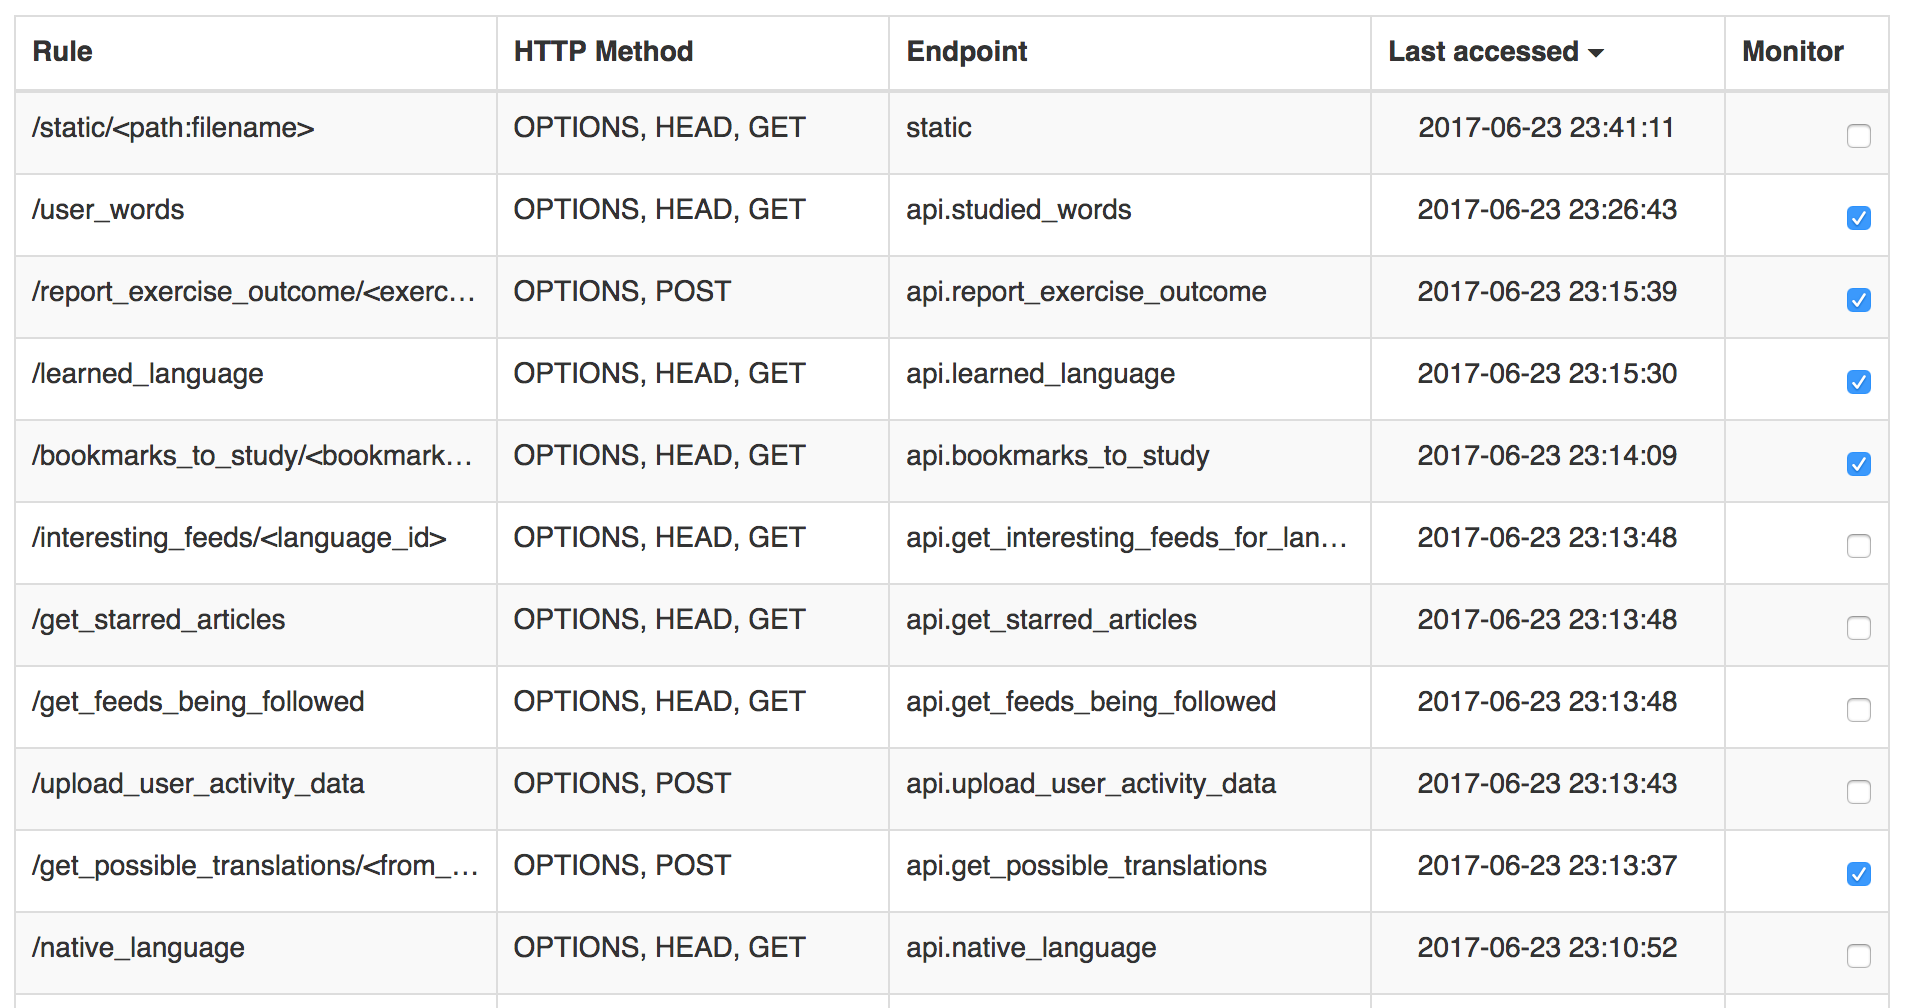
\includegraphics[width=0.8\linewidth]{selecting_endpoints.png}
      \caption{All of the endpoints of the Zeeguu app are shown such that a selection can be made for monitoring them}
      \label{fig:sep}
    \end{figure}

  In order to monitor an endpoint, the \tool creates a function wrapper for the API function that corresponds to the endpoint. This way, the wrapper will be executed whenever that API call is made. The wrapper contains the code that takes care of monitoring an endpoint. Data collected by the wrappers are persisted in a local database.

  There are two main categories of visual perspectives that are available using \tool:
  \begin{enumerate}
    \item \textit{Overviews} that present information and measurements about all the endpoints of interest, and
    \item \textit{Detailed information} about the measurements pertaining to a specific endpoint.
  \end{enumerate}

  In the remainder of the paper we present several of these perspectives.\footnote{We recommend obtaining a color version of this paper for better readability}

  % The second endpoint conists of two parts, one of them being a table that shows for every monitored endpoint the number of hits it has gotten, the time it was last accessed and its average execution time. The second part is a view with four graphs which show:
  % \begin{itemize} 
  %   \item A heatmap of the total number of requests to the monitored endpoints
  %   \item A stacked bar chart that shows the total number of requests to the monitored endpoints per endpoint per day
  %   \item A boxplot graph showing the average execution time per version of the web service
  %   \item A boxplot graph showing the average execution time for every monitored endpoint
  % \end{itemize}


%!TEX root=vissoft.tex

\section{Service Utilization}
\label{sec:util}

  The most fundamental insight that a service maintainer needs regards service utilization. \vspace{0.5cm}

  Figure \ref{fig:aeu} shows a first perspective on endpoint utilization that \tool provides: a stacked bar chart of the number of hits to various endpoints grouped by day  shows that at its peak the API has about 2500 hits per day. 
  The way users interact with the platform can also be inferred since the endpoints are indicators of different activity types, e.g.: 

  \begin{enumerate}

    \item {\color{myblue}\epTranslations} is an indicator of the amount of foreign language reading the users are doing

    \item {\color{myviolet} \epOutcome} is an indicator of the amount of foreign vocabulary practice the users are doing

  \end{enumerate}


  \begin{figure}[!ht]
    \centering
    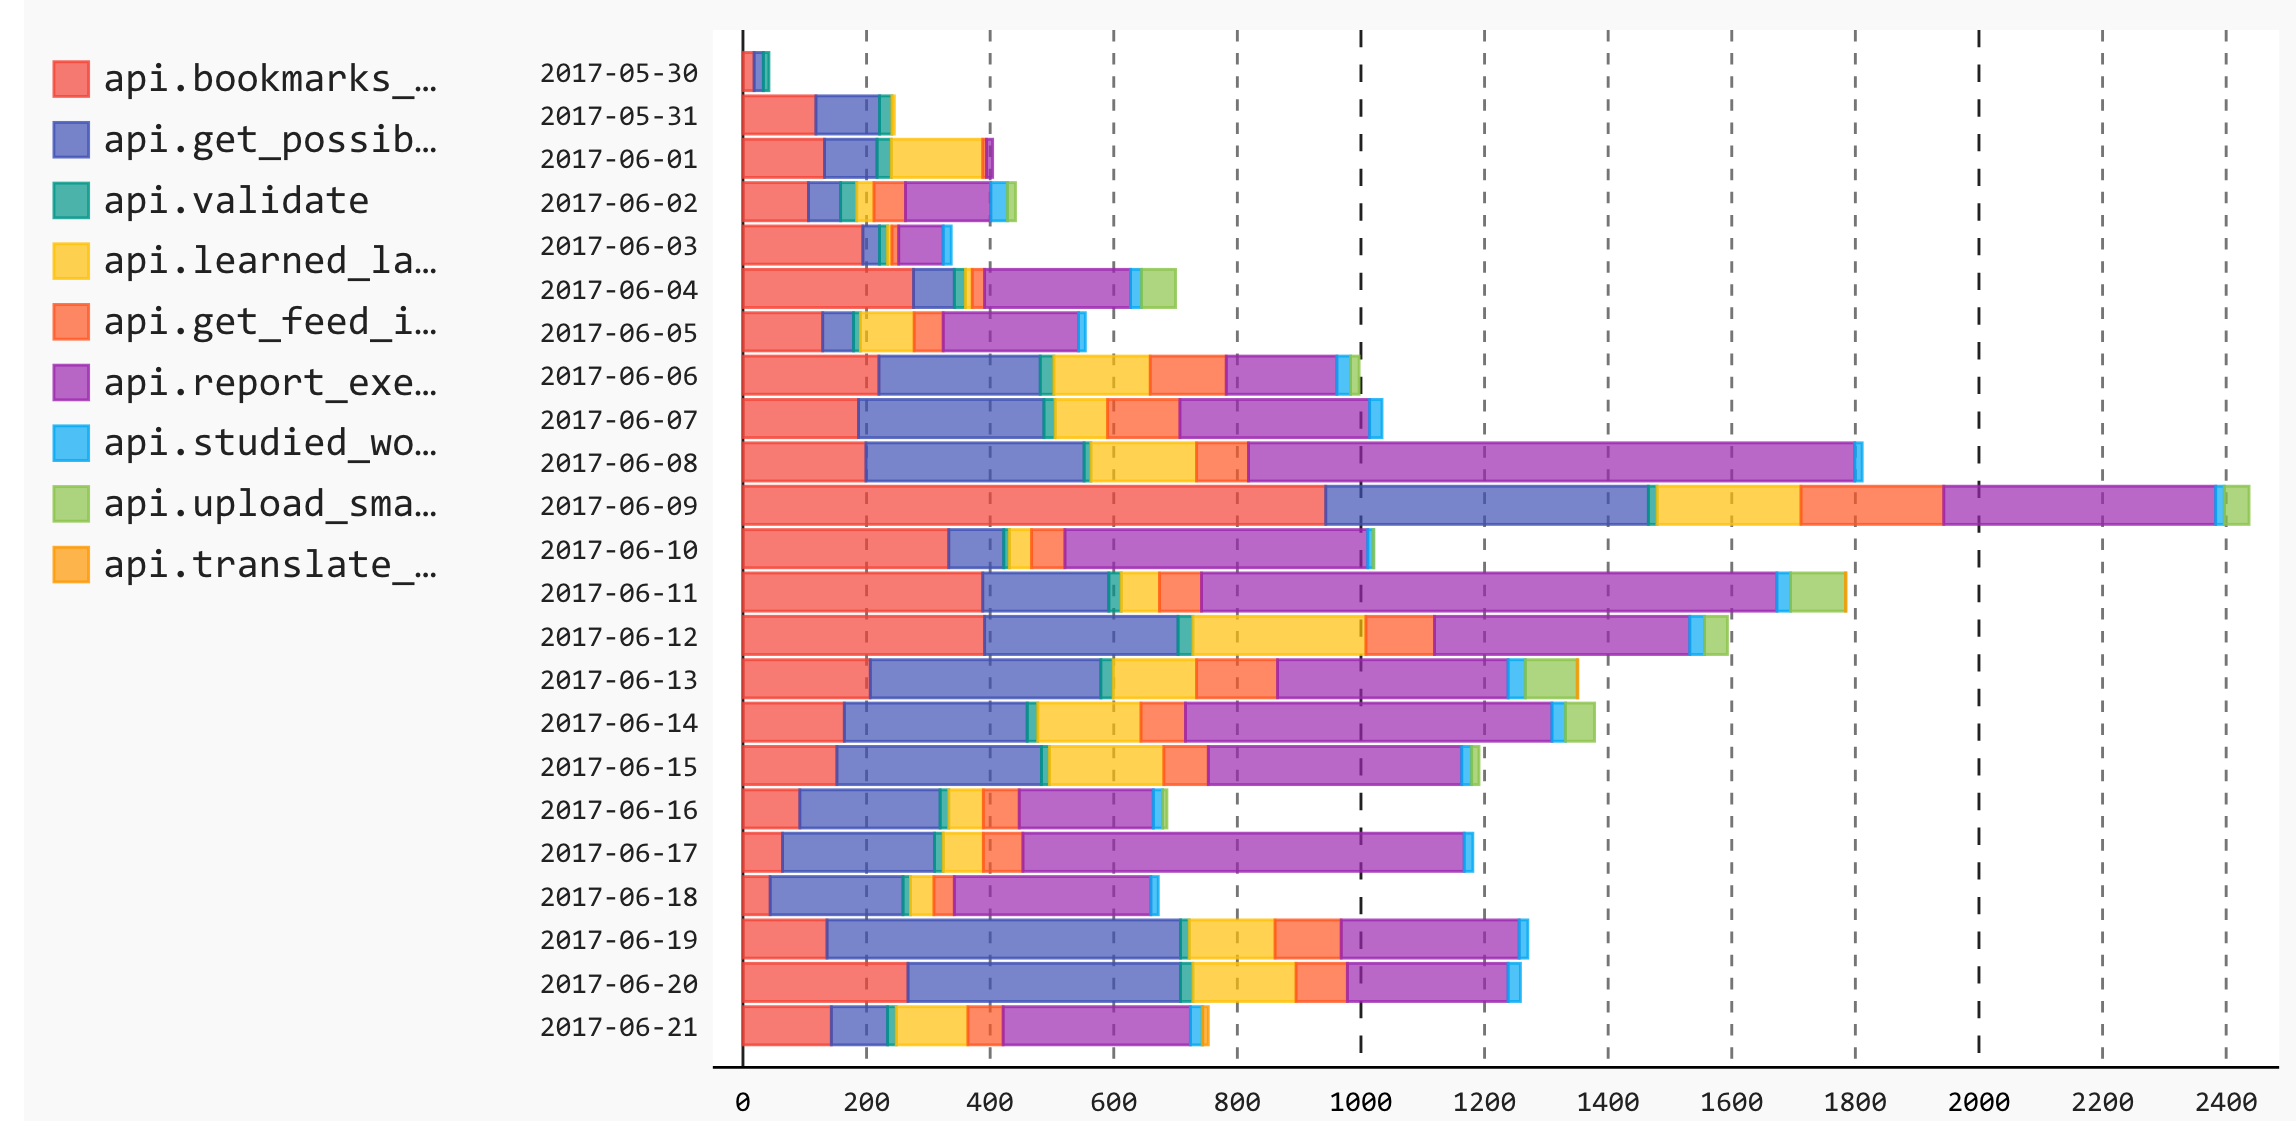
\includegraphics[width=\linewidth]{all_endpoints_usage.png}
    \caption{The number of requests per endpoint per day view shows the overall utilization of the monitored application}
    \label{fig:aeu}
  \end{figure}

  Besides showing the overall utilization, this endpoint provides to the maintainer with information relevant for decisions regarding endpoint deprecation -- one of the most elementary ways of {\em understanding the needs of the downstream}\cite{Haen14a}. In our case study, the maintainer realized that several endpoints which they thought were not being used, contrary to their expectations, were actually being used.\footnote{Usage information can also be used to increase the confidence of the maintainer that a given endpoint is not used, although it can never be used a proof.}

  \niceseparator

   \todo{Add the time series graph and discuss it before the heatmap? We can then sell the heatmap better} 
   \ml{Not sure about which graph you refer to here V}

  A second type of utilization question that the \tool can answer automatically regards {\em cyclic patterns of usage per hour of day}. 

  % \mltp{ can we add vertical lines that highlight the beginning of a new week (e.g. before Sunday): }
  % Patrick: adding separators in the graph is unfortunately not supported by the library.

    \begin{figure}[!ht]
      \centering
      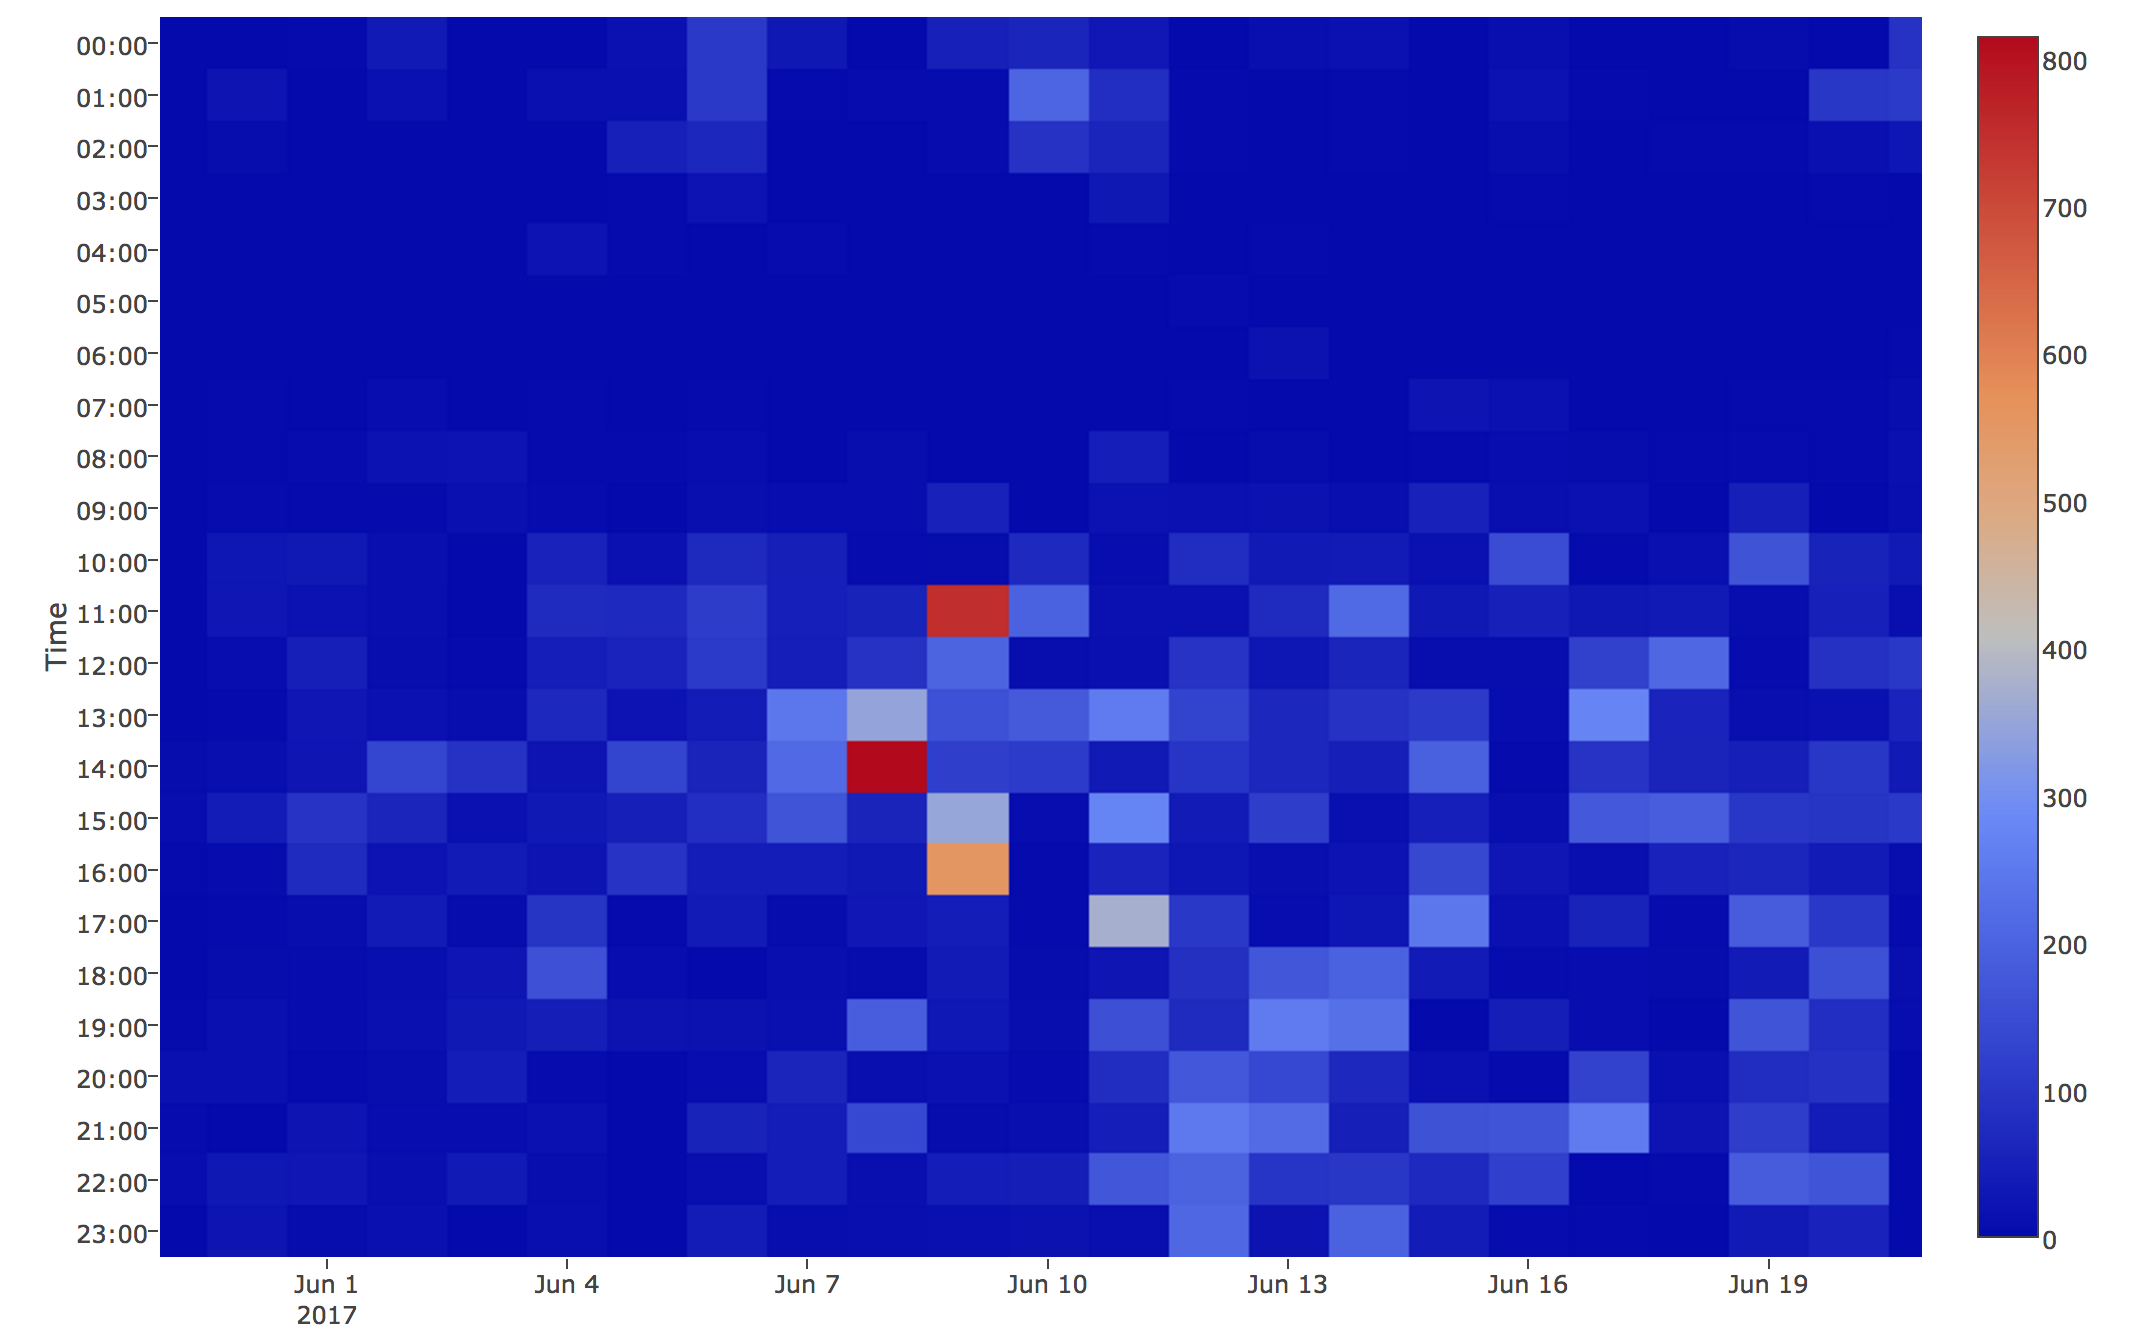
\includegraphics[width=\linewidth]{daily_patterns}
      \caption{Usage patterns become easy to spot in the requests per hour heatmap}
      \label{fig:dp}
    \end{figure}


  Figure \ref{fig:dp} shows the the API not being used during the early morning hours, and that most of the activity focused around working hours and some light activity during the evening. This is consistent with the fact that the current users are all in the central european timezone. 




\section{Endpoint Performance}
\label{sec:perf}

  The \tool also collects information regarding endpoint performance. The view in \Fref{fig:ep} summarizes the response times for various endpoints by using a box-and-whiskers plot. 

  % \ml{Thijs and Patrick... the visualization people will complain when they see that we have different colors for the same endpoint in different graphs. Can we insure that there is consistency in colors? Simplest trick would be to obtain the color by hashing the name of the endpoint... in that case the same endpoint would have the same color in various graphs.}
  % This is supported in the latest version of the dashboard

  \begin{figure}[!ht]
    \centering
    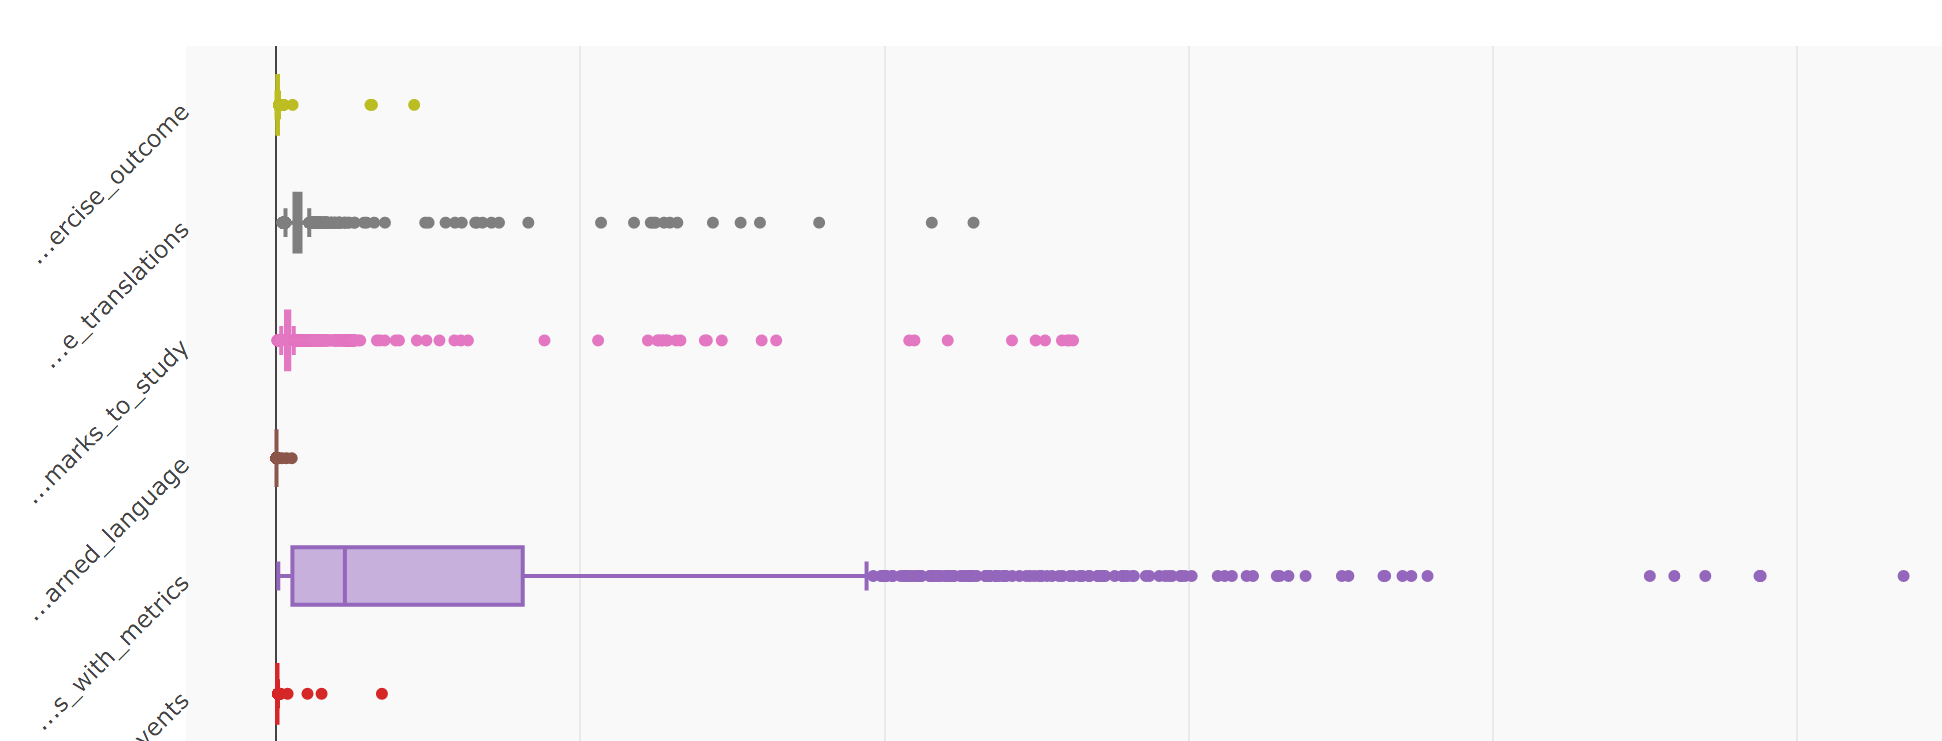
\includegraphics[width=0.9\linewidth]{endpoint_performance_}
    \caption{The response time (in ms) per monitored endpoint view allows for identifying performance variability and balancing issues}
    \label{fig:ep}
  \end{figure}

  After investigating this view it became clear to the maintainer that three of the endpoints had very large variation in performance.   The most critical for the application and consequently the one optimized first was the \epTranslations endpoint which was part of an interactive loop in the reader applications that relied on the Zeeguu API. 


  \niceseparator

  However, with the current configuration of the tool, it would be impossible for the maintainer to see the improvements resulting from the optimization. One way to do this is to add an extra line of configuration to \tool find the git\footnote{\url{https://git-scm.com/}} folder of the deployed service: 

%  \begin{lstlisting}[caption=Configuring the \tool with the path to the .git folder enables the generation of evolutionary performance graphs, style=custompython]
%
%dashboard.config.git = 'path/to/.git'
%
%
%    \end{lstlisting}
    
    \begin{lstlisting}[style=custompython]
  
  dashboard.config.git = 'path/to/.git'
    
  \end{lstlisting}  
 
  With this extra configuration, the dashboard can now automatically detect the current version of the project, and group measurements by version. \tool can now generate the view in \Fref{fig:tee} where the performance of a given endpoint is tallied by version\footnote{Alternatively, the maintainer can add version identifiers manually for the web application through a configuration file if the system does not use git.}
  
  
    \begin{figure}[h!]
      \centering
      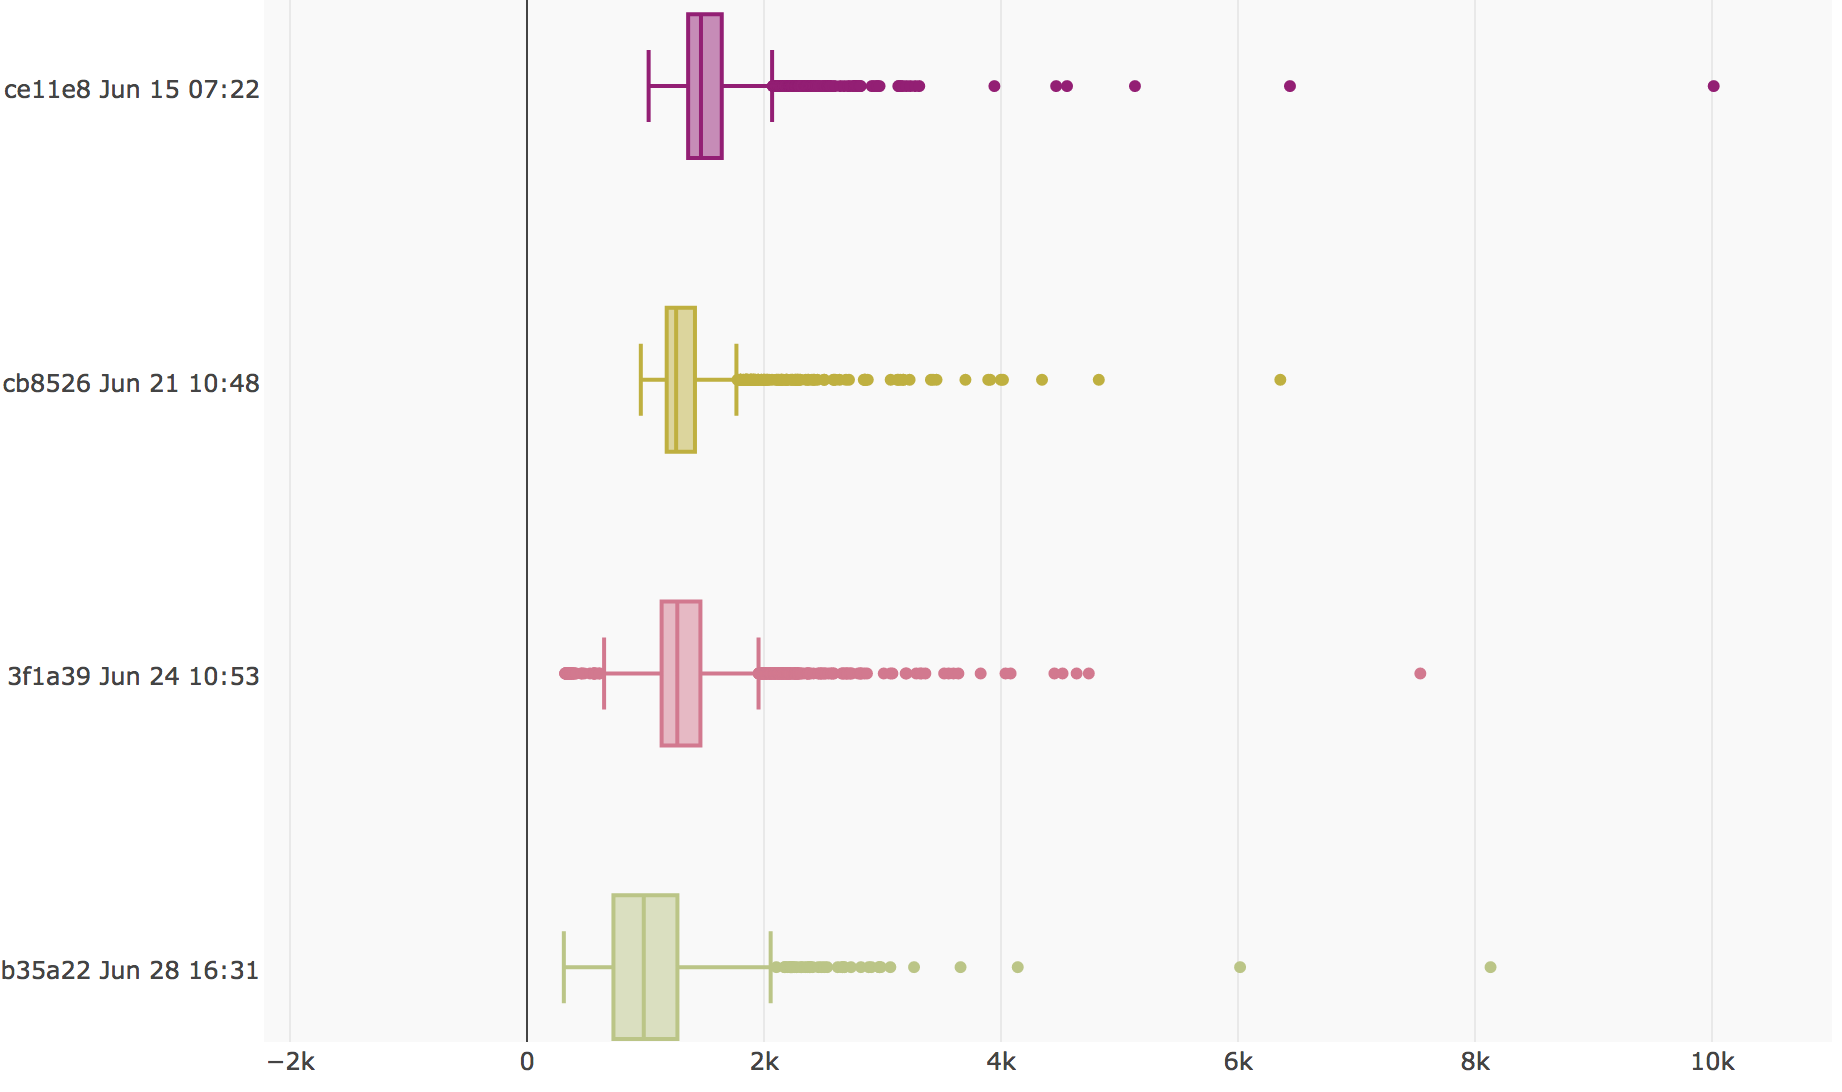
\includegraphics[width=\linewidth]{translation_endpoint_evolution_}
      \caption{Visualizing The Performance Evolution of the \epTranslations endpoint}
      \label{fig:tee}
    \end{figure}

  This way the maintainer could confirm that the performance of the translation endpoint improved: in the latest version (bottom-most box plot in \Fref{fig:tee}) the entire box plot moved to the left and there are fewer outliers.


  \niceseparator

  The \tool collects {\bf extra information about such outliers}: Python stack trace, CPU load, request parameters, etc. in order to allow the maintainer to investigate the causes of these exceptionally slow response times. 

  In order to address this, but without degrading overall performance, the \tool tracks for every endpoint a running average value. When it detects that a given request is an outlier with respect to this past average running value, it triggers the {\em outlier data collection routine} which stores all the previously listed extra information about the current execution environment. 

\newpage
\section {User Experience}
\label{sec:user}

  For service endpoints which run computations in real time, the maintainer of a system must understand the endpoint performance on a per-user basis, especially for situations where the system response time is a function of some individual user load\footnote{E.g. in GMail some users have two emails while other have twenty thousand and this induces different response times for different users}.
%
  The \tool provides a way of grouping information on a per user basis. However, to do this, the developer must specify the way in which a given API call can be associated with a given user. There are multiple ways, the simplest of which utilizes again the common expectations of Flask applications that offers a global \code{request} object which contains a \code{session} object which encapsulates information: 

  %\begin{lstlisting}[float,caption=Simply define a custom app-specific function for user retrieval and pass it to the \tool to group information by user,style=custompython]
  \begin{lstlisting}[style=custompython]  
    # app specific way of extracting the user
    # from a flask request object    
    def get_user_id(request):
      sid = int(request.args['session'])
      session = User.find_for_session(sid)
      return user_id

    # attaching the get_user_id function
    dashboard.config.get_group_by = get_user_id

  \end{lstlisting}

  In the Zeeguu case study, one of the slowest endpoints, and one with the highest variability as shown in \Fref{fig:ep} is \epFeedItems: it retrieves a list of recommended articles for a given user. However, since a user can be subscribed to anything from one to three dozen article sources, and since the computation of the difficulty is personalized and it is slow, the variability in time among users is likely to be very large. 


  Figure \ref{fig:tpu} shows some of the results of calling the \epFeedItems endpoint for various users. The figure shows that the response times for this endpoint can vary considerably for different users. 

  \begin{figure}[!ht]
    \centering
    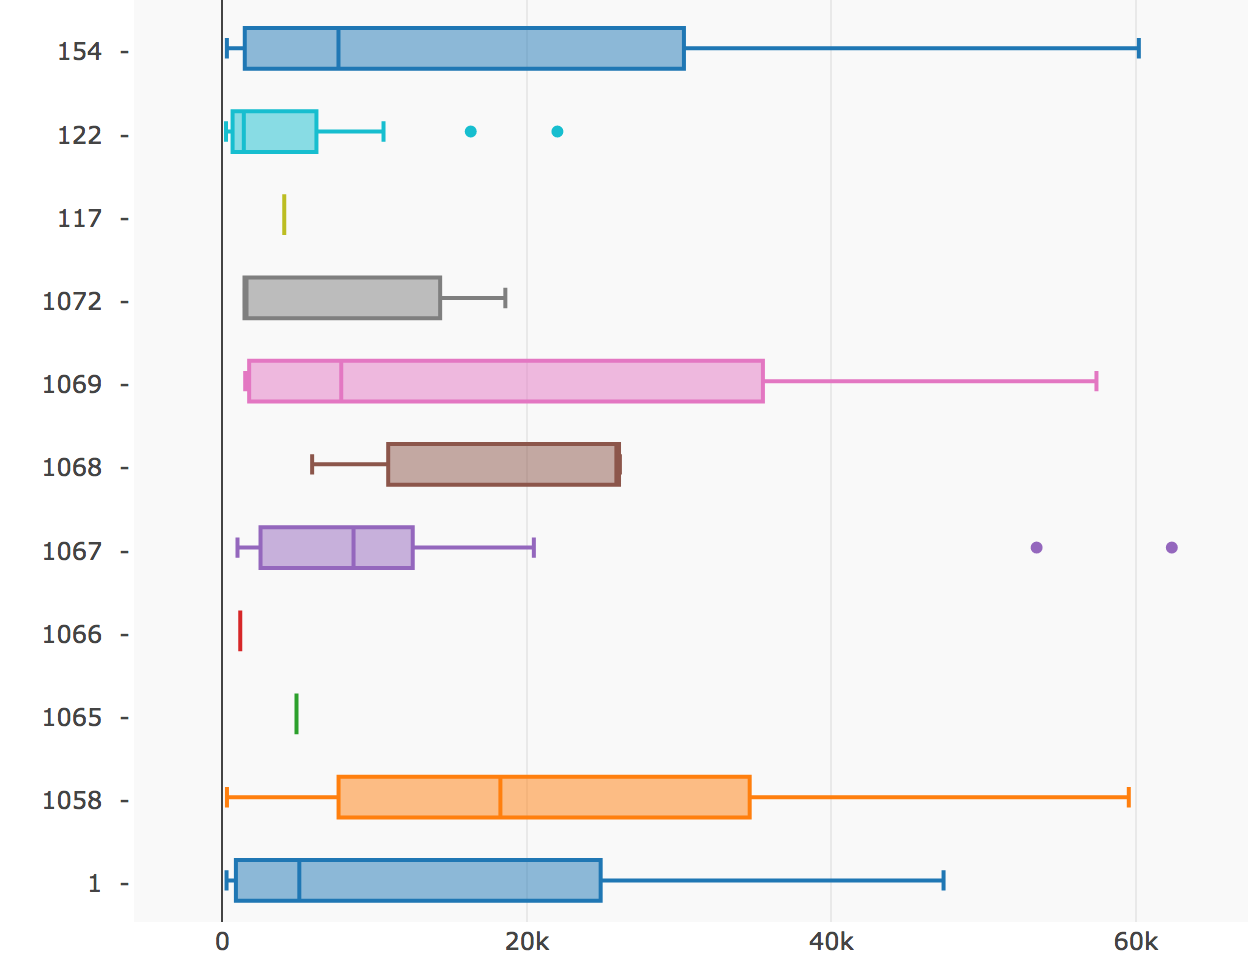
\includegraphics[width=\linewidth]{time_per_user}
    \caption{The \epFeedItems shows a very high variability across users}
    \label{fig:tpu}
  \end{figure}

  \newpage
  \niceseparator

  The limitation of the previous view is that it does not present the information also on a per version basis. To address this, a different visual perspective entitled \perspective{Evolving per-User Performance} can be defined. Figure \ref{fig:tuv} attempts to present the information that would be required in such an perspective. 

  \begin{figure}[!ht]
    \centering
    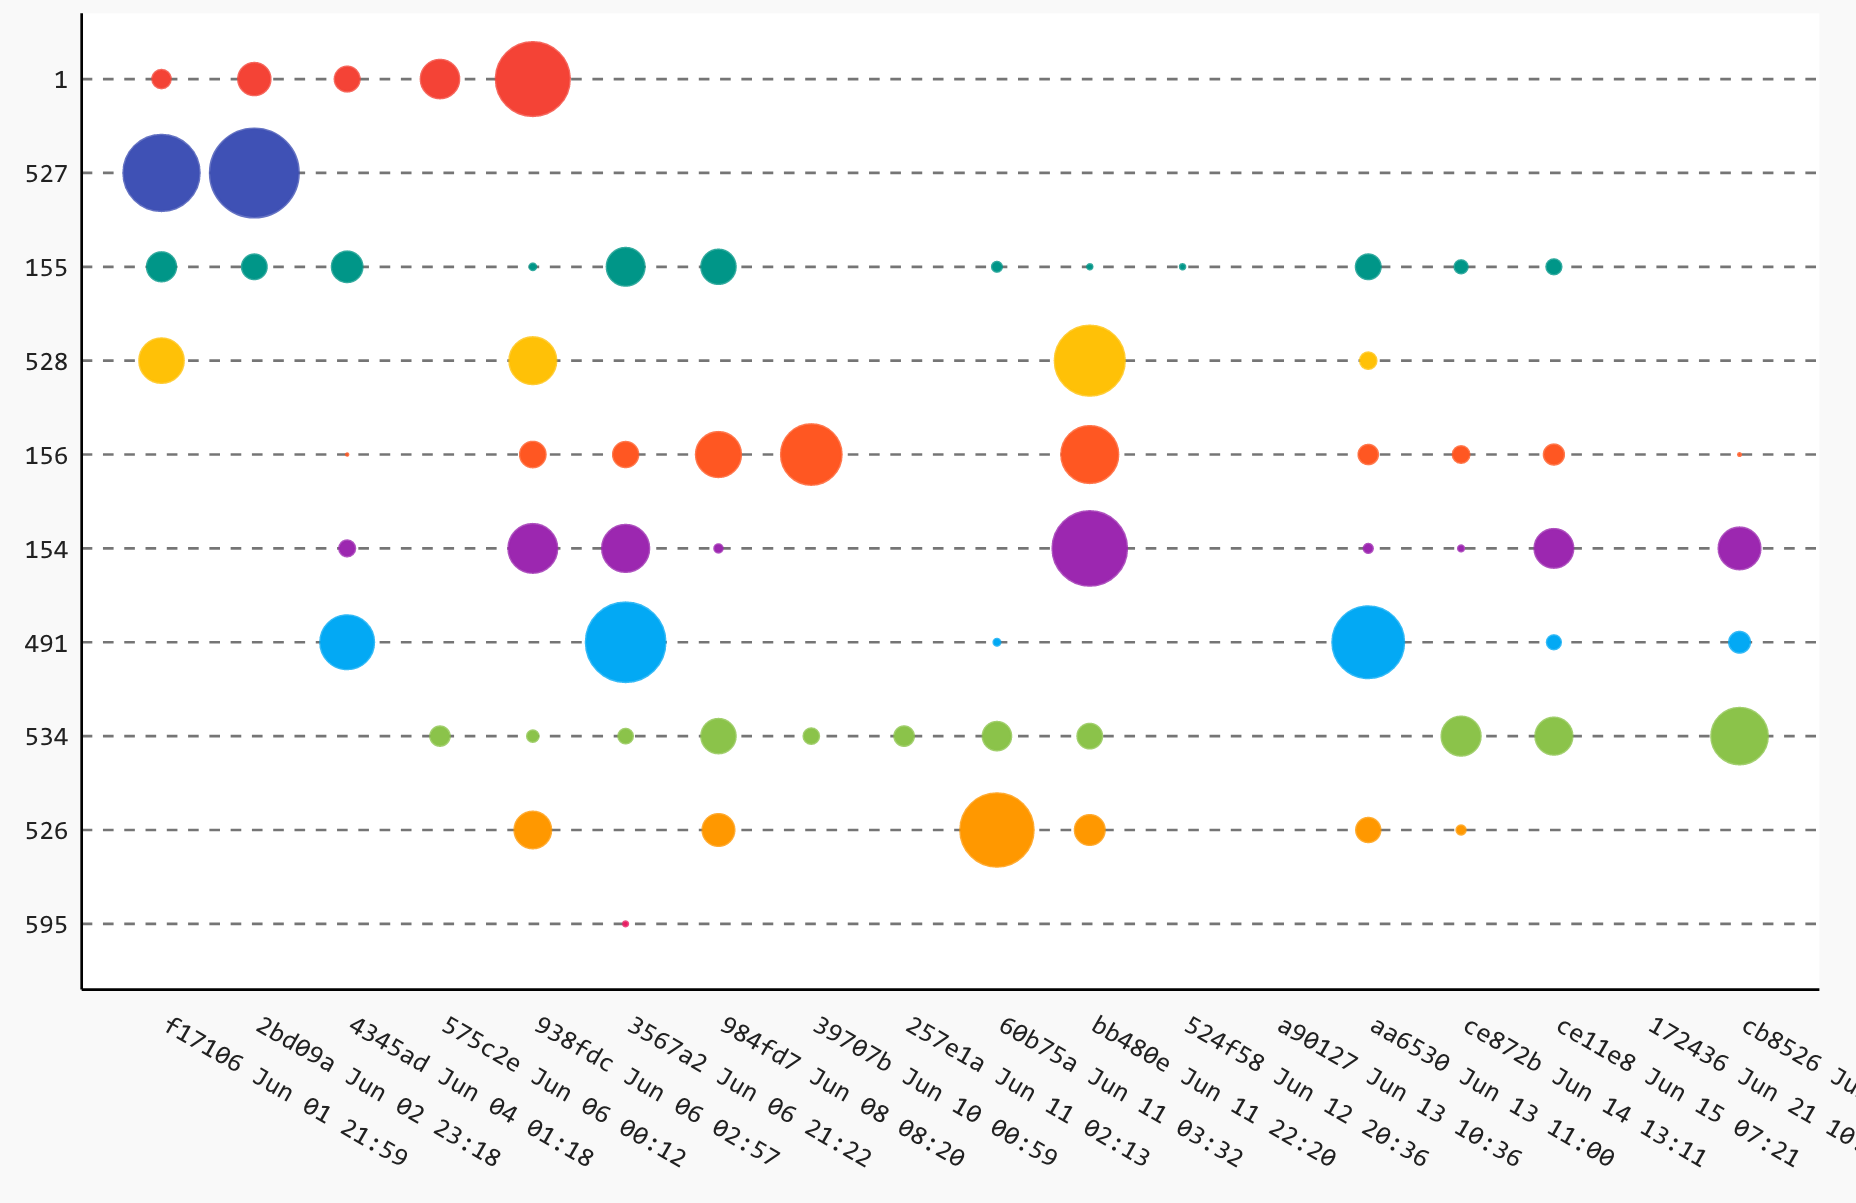
\includegraphics[width=\linewidth]{time_per_user_per_version}
    \caption{This perspective shows that the evolution of response times for individual users (horizontal lines) across versions (the x-axis)}
    \label{fig:tuv}
  \end{figure}

  For the situations in which the user information is not available, the \tool also tracks out of the box information about different IPs. In some cases this might be a sufficiently good approximation of the user diversity and identity. 
  
  In the interest of space limitations we are not showing this, and quite a few more visualizations provided by the \tool. The interested reader is referred to \Sref{sec:install} for further information on how to install the tool and how to get access to the data of the case study.

\section{Discussion}

  \subsection{Automatically Monitoring System Evolution}

  The main goal of the \tool design was to allow analytics to be collected and insight to be gained by making the smallest possible changes to the running API. %To allow the collection of evolutionary information 
%
  This technique assumes that the web application code which is the target of the monitoring is deployed using \git in the following way: 

  \begin{enumerate}
    \item The deployment engineer pulls the latest version of the code from the integration server; this will result in a new commit being pointed at by the HEAD pointer. %than previously
    \item The deployment engineer restarts the new version of the service. At this point, the \tool detects that a new HEAD is present in the local code base and consequently starts associating all the new data points with this new commit\footnote{The \tool detects the current version of the analyzed system the first time it is attached to the application object, and thus, assumes that the Flask application is restarted when a new version is deployed. This is in tune with the current version of Flask, but if the web server will support dynamic updates in the future, this might have to be taken into account}.
  \end{enumerate}

  The advantage of this approach is the need for minimal configuration effort, as discussed in the presentation of the tool. The disadvantage is that it will consider on equal ground the smallest of commits, even one that modifies a comment, and the shortest lived of commits, e.g.~a commit which was active only for a half an hour before a new version with a bug fix was deployed, with major and minor releases of the software. %as a distinct way of grouping the data points. 
  A mechanism to control which versions are important for monitoring purposes is therefore required to be added.
%
  A further possible extension point here is supporting other version control systems (e.g. Mercurial). However, this is a straightforward extension.



  \subsection{User-Awareness }

    User awareness as presented in Section \ref{sec:user} is useful, but the scalability of the approach must be taken into consideration. In our case study we had about several hundreds users (of which about \activeUserCount were active during the course of the study). However, different perspectives might be required for APIs with millions of users.


  \subsection{Other Possible Groupings}

    There are other groupings of service utilization and performance that could be important to the maintainer, that we did not explore in this paper. For example, if the service is using OAuth, then together with every request, in the header of the request there is information about the application which is sending a request. Grouping the information by application that sends the request could be important in such a context. In general, providing a mechanism that would allow very easy specification of groupings (either as code annotations, as normal code, or as configuration options) is an open problem that \tool and any other similar library will have to face.

  \subsection{Tool and Source Code Availability}
  \label{sec:install}

    The images in this paper are screenshots of the interactive visualizations from the deployment of \tool in the context of the Zeeguu core API. The actual deployment can be consulted online by the reviewers and readers of this article\footnote{\url{https://zeeguu.unibe.ch/api/dashboard}; username: {\em guest}, password: {\em vissoft}}.

    \tool is implemented for Python 3.6 and is available on the Python Package Index repository\footnote{\url{https://pypi.python.org/pypi/flask-monitoring-dashboard/1.8}} from where it can be installed on any system that has Python installed by running \install from the command line. 

    The source code of the \tool is published under a permissive MIT license and is available on GitHub\footnote{\url{https://github.com/mircealungu/automatic-monitoring-dasboard}}.



\section{Related Work}
\label{sec:related}

There is a long tradition of using visualization for gaining insight into software performance. Tools like Jinsight \cite{Pauw02a} and Web Services Navigator \cite{Pauw05} pioneered such an approach for Java and for Web Services that communicate with SOAP messages. Both have an ``omniscient'' view of the services / objects and their interactions. As opposed to them, in our work we present an analytics platform which focuses on monitoring a single Python web service from its own point of view.

From the perspective of service monitoring, our work falls within the server-side run-time monitoring of services ~\cite{ghezzi2007run}. While we don't implement the more advanced features of related monitoring solutions like QoS policies driving the monitoring, it presents nevertheless an easy to use approach support improving the performance of web applications. 

% \va{Mircea: Consider removing the rest for space...}
% An existing monitoring tool is Pingdom \footnote{https://www.pingdom.com/company/why-pingdom}, which monitors the uptime of an existing web-service. This tool works by pinging the websites (up to 60 times) every minute automatically. Thus this creates a lot of overhead and is bound to be noisy since it will also be influenced by the speed of the network connection\footnote{Another problem is that such a tool would }

% \todo{Runscope? Others?}


\section{Conclusion and Future Work}

In this paper we have shown that it is possible to build a low-effort monitoring solution which provides plenty of feedback to a user with very little effort. The user group that we are aiming for with this work is application developers using Flask and Python to build web applications with limited or no budget for implementing their own monitoring solutions. The emphasis is in allowing such users to gain insight into how the performance of the service evolves together with the application itself.

In the future, we plan to perform case studies with other sytstems, with the goal of discover other needs and to wean out the less useful visualizations in the \tool. We plan to also extend the tool towards supporting multiple deployments of the same applications across multiple nodes (e.g. for the situations where the application is deployed together with a load balancer). Finally, we plan to integrate \tool with unit testing as a complementary source of performance evolution.

% references section

\bibliographystyle{IEEEtran}
\bibliography{vissoft}


% that's all folks
\end{document}


